Beskrivning av kunskapsläget (detta är ett obligatoriskt moment i din rapport). Inom vilket område skall du redogöra för kunskapsläget? Om ditt projekt t.ex. handlar om att ta fram ett gränssnitt kan du välja att redogöra för kunskapsläget inom användargränssnitt – vad kännetecknar ett bra gränssnitt, vilka tester/undersökningar har gjorts, etc. Om ditt projekt t.ex. handlar om att implementera en specifik sak i VHDL är det lämpligt att du redogör för varför VHDL är speciellt lämpligt att använda, vilka andra alternativ som finns och fördelar samt nackdelar för olika alternativ. (Denna del, ”beskrivning av kunskapsläget”, är ett moment som högskolan kräver i projektet som ett prov på er förmåga att inhämta och sammanställa kunskap.)\medskip
 
Den Raviolimaskinen som är tänkt att utvecklas för detta projekt består av några viktiga delar. Det består av en pump som ska pumpa fram Raviolis ifyllnings materialet på degen. För detta måste man redogöra hur en pump fungerar, vilkar delar en pump har och hur man ska designa det för att det ska passar just detta projekt.\medskip

En annan del ska vara degformen. På figuren ~\ref{degfrom} visas en degform som används för att knyta degen manuellt genom att trycka på formens sidor. För detta projekt har funderats på att utveckla en degform som kan styras med en eller två motorer. En viktig uppgift är att överföra motorers rörelseenergi till degformen på ett sätt att den får nog kraft för att knyta degen. Det kommer finnas kugghjul för energiöverföringen från motor till degformen. Kunskapen inom olika typer av kugghjul och hur ett kugghjul fungerar ska utvecklas.\medskip

\begin{figure}[h]
	\begin{center}
		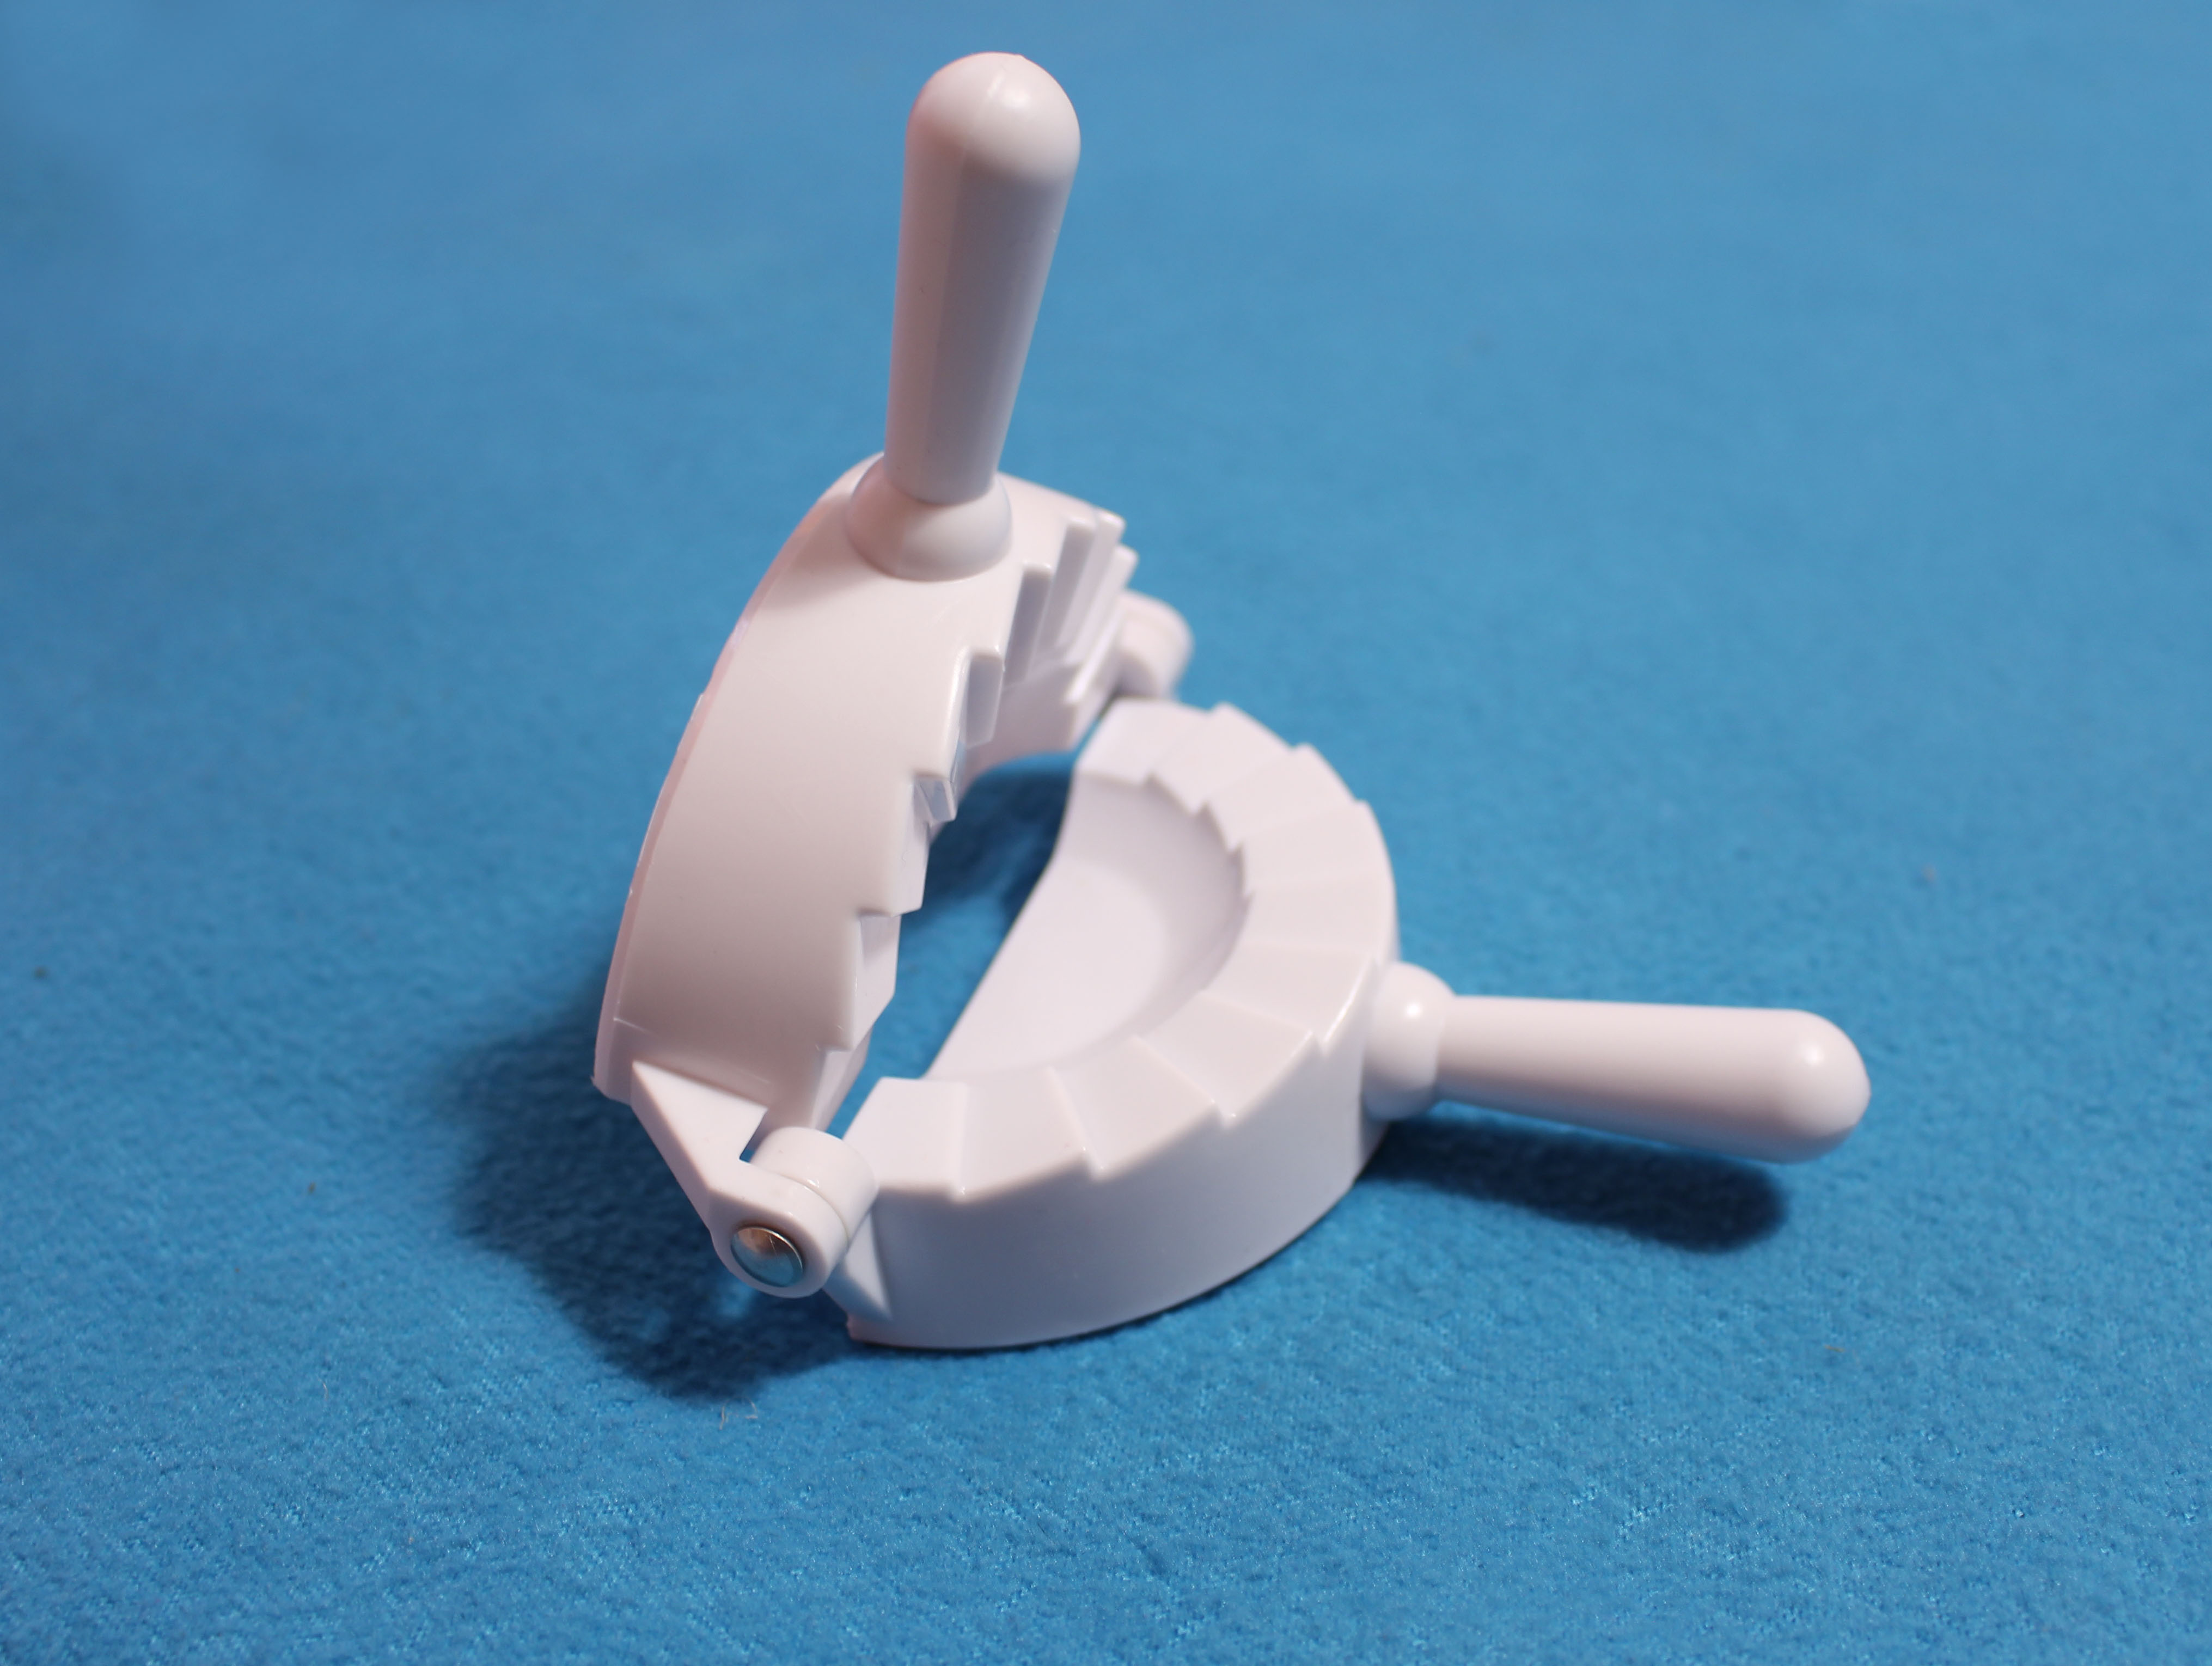
\includegraphics[scale=0.08] {images/degform.jpg}
		\caption{Degform för manuell ifyllning}
		\label{degfrom}	
	\end{center}
\end{figure}\medskip

För att alla Raviolimaskinens delar ska fungera ihop och varje del gör sin uppgift i rätt tid, måste det en enhet för att kontrollera dem. Kontrol av alla delar görs m.h.a. en mikrokontroller som bestämmer vad som ska hända i varje tidspunkt. Olika typer av mikrokontroller måste analyseras för att hitta den som passar bäst till projektet.




